\documentclass[conference]{IEEEtran}
\IEEEoverridecommandlockouts

\usepackage{cite}
\usepackage{amsmath,amssymb,amsfonts,amsthm}
\usepackage{algorithm}
\usepackage{algpseudocode}
\usepackage{graphicx}
\usepackage{textcomp}
\usepackage{xcolor}
\usepackage{booktabs}
\usepackage{url}
\usepackage[hidelinks]{hyperref}

\newtheorem{definition}{Definition}
\newtheorem{proposition}{Proposition}
\newtheorem{lemma}{Lemma}
\newtheorem{remark}{Remark}
\newtheorem{assumption}{Assumption}

\newcommand{\R}{\mathbb{R}}
\newcommand{\N}{\mathbb{N}}
\newcommand{\W}{\mathcal{W}}
\newcommand{\Obs}{\mathcal{O}}
\newcommand{\Rob}{\mathcal{R}}
\newcommand{\Cand}{\mathcal{C}}
\newcommand{\Bod}{\mathcal{B}}
\newcommand{\X}{\mathcal{X}}
\newcommand{\Uc}{\mathcal{U}}
\newcommand{\clr}{\varepsilon}

\begin{document}

\title{Unsatisfiability as a Coordination Signal:\\
Core-Guided B-Spline Repair for Multi-Robot\\
Kinodynamic Motion Planning}

% TODO: fill in the author block before submission. Square brackets must stay braced
% here -- a bare [ after \\ is parsed as the optional length argument of \\.
\author{\IEEEauthorblockN{{Author Name}}
\IEEEauthorblockA{\textit{{Department}} \\
\textit{{Institution}} \\
{City, Country} \\
{email@institution.edu}}
}

\maketitle

\begin{abstract}
Multi-robot kinodynamic planners resolve inter-robot conflicts reactively: a collision is
observed between a specific pair of trajectories, and that pair is re-planned. The trigger
is therefore an \emph{instance} of failure, and the repair it licenses is local to the two
robots that happened to touch. We replace that trigger with a \emph{proof}. Each robot owns
a growing finite set of candidate motions, each of which is a cubic B-spline given a
time-optimal speed profile and driven through the exact flatness inverse of the
second-order unicycle, so every candidate is admissible in isolation by construction.
A~SAT solver selects one candidate per robot; pairwise collision clauses are added lazily,
only for the combinations the solver actually proposes. When the solver reports
\textsc{unsat}, its \emph{unsatisfiable core} is a certificate that the current candidate
sets admit no joint selection at all, and it names both the robots responsible and the
workspace points at which their candidates met. That certificate drives repair: control
points of the blamed splines within a bounded neighbourhood of a contested point are
displaced perpendicular to the curve. Because a cubic B-spline basis function is supported
on four knot spans, the edit is provably confined to a bounded stretch of the curve --- on
our worked instance, three of nineteen control points move and $4.78$\,m of a $15.00$\,m
curve changes, with the rest bit-identical --- so repair is additive rather than
destructive and the learned clause database is never invalidated. We give the construction
in full, with every definition, and illustrate the complete loop on a four-robot instance
that the method solves in three rounds, $186$ pairwise checks and zero resampling
fallbacks, returning a plan the simulator's own collision checker verifies at
$0.079$\,m of surface clearance.
\end{abstract}

\begin{IEEEkeywords}
multi-robot systems, kinodynamic motion planning, satisfiability modulo theories,
B-splines, conflict resolution
\end{IEEEkeywords}

\section{Introduction}

A multi-robot kinodynamic planner has to answer two questions that pull in opposite
directions. The first is a continuous question --- \emph{what motion does robot $i$
execute?} --- and it is answered by machinery that knows about acceleration bounds,
curvature limits and obstacle geometry. The second is a combinatorial question ---
\emph{which of the possible motions do the robots execute together?} --- and it is answered
by machinery that knows about mutual exclusion. Most planners in this space, including
K-ARC \cite{karc2025}, db-CBS \cite{dbcbs2024} and db-LaCAM \cite{dblacam2025}, answer the
second question by repeatedly re-asking the first: a conflict is found, a constraint is
imposed, and a continuous planner is invoked again.

This paper is about changing what the combinatorial layer is allowed to say back. In a
conflict-driven planner the signal returned by the combinatorial layer is always of the
form ``\emph{these two trajectories touch}''. It is an existential statement about one
observed failure. A solver over a finite candidate set can return something strictly
stronger: ``\emph{no selection from these candidate sets works, and here is the subset of
refutations that already makes it impossible}''. That is a universal statement over the
entire candidate set, and it is available at no extra cost, because it is exactly what a
modern SAT solver produces when it proves unsatisfiability under tracked assumptions
\cite{z3}.

The difficulty is that such a certificate is useless unless the geometry layer can act on
it. A certificate says \emph{which} robots are jointly stuck and \emph{where} their motions
met. Acting on it means editing a motion near a named workspace point without disturbing
the rest --- because the rest of that motion is already encoded in dozens of learned
clauses that would otherwise have to be thrown away. This is precisely the property a
B-spline has and a sampled polyline does not: local support. A cubic basis function is
nonzero on four knot spans, so displacing a control point edits a bounded arc and leaves
the remainder of the curve unchanged, bit for bit.

\subsection*{Contributions}

\begin{enumerate}
  \item A complete formulation in which the coordination decision is a Boolean selection
        problem over per-robot candidate sets, with collision clauses added lazily and
        tracked, so that unsatisfiability yields a core (Sec.~\ref{sec:encoding}).
  \item A repair operator driven by that core rather than by an observed pairwise
        collision, with a locality guarantee inherited from the B-spline basis
        (Sec.~\ref{sec:repair}), and the measurement of that locality on a real instance.
  \item A candidate realisation pipeline in which admissibility under the true
        second-order bounds holds by construction, via differential flatness and a
        time-optimal path parameterisation, with no boundary-value problem and no
        trajectory optimiser in the loop (Sec.~\ref{sec:realise}).
  \item A fully worked four-robot instance carried through every stage of the algorithm
        with the actual numbers produced by the implementation (Sec.~\ref{sec:example}),
        and an explicit statement of the soundness gap the discrete-time collision
        semantics leaves open (Sec.~\ref{sec:properties}).
\end{enumerate}

\section{Related Work}

\paragraph*{Conflict-driven multi-robot planning}
Conflict-Based Search \cite{cbs2015} established the two-level pattern: a low level plans
for one agent, a high level branches on an observed conflict. db-CBS \cite{dbcbs2024} and
db-LaCAM \cite{dblacam2025} carry it into kinodynamic settings by composing
discontinuity-bounded motion primitives. K-ARC \cite{karc2025} builds a sub-problem around
each conflicting \emph{pair} and grows it reactively when resolving one conflict spoils
another. In all of these the unit of blame is a pair, and the repair discards and replaces
the offending motions.

\paragraph*{SAT and SMT encodings}
Surynek \cite{surynek2020} gives the closest methodological precedent: a lazy SMT encoding
for continuous multi-agent path finding in which collision constraints are added on demand
rather than eagerly. The structural difference here is what happens on
\textsc{unsat}. In \cite{surynek2020} the candidate structure is a fixed roadmap, so
unsatisfiability under a makespan bound is resolved by raising the bound. In our setting the
candidate sets are themselves the object being refined, so unsatisfiability is a statement
about the \emph{geometry we generated}, and the core tells us which piece of geometry to
regenerate.

\paragraph*{B-splines in robot motion planning}
B-splines are standard practice for trajectory representation in aerial robotics. Usenko
\emph{et al.} \cite{usenko2017} replan uniform B-splines in real time against a circular
buffer; Fast-Planner \cite{fastplanner2019} and EGO-Planner \cite{egoplanner2021} optimise
control points directly, the latter by pushing a colliding segment away from an obstacle
using a collision-free guide path; EGO-Swarm \cite{egoswarm2021} extends this to a swarm.
Elbanhawi \emph{et al.} \cite{elbanhawi2015} survey the use of B-splines for continuous
path smoothing on car-like robots. Our repair operator is deliberately the same geometric
move as \cite{egoplanner2021} --- displace the control points near a contested point --- but
it is driven by a proof of joint infeasibility rather than by a gradient, and the
displacement is applied to the robots a core names rather than to the robot that observed
the obstacle.

\paragraph*{Trajectory realisation}
Differential flatness has been used to avoid boundary-value problems in trajectory
generation since \cite{mellinger2011}. Time-optimal path parameterisation under actuator
bounds is a classical problem with a modern reachability-based solution in TOPP-RA
\cite{toppra2018}; we use the simpler forward--backward sweep, which is sufficient for the
single tangential-acceleration bound we carry. For continuous-time inter-robot safety
certificates, Park and Kim \cite{parkkim2020} bound the relative trajectory of a pair by
the convex hull of its relative Bernstein coefficients; we discuss this in
Sec.~\ref{sec:properties} as the principled fix for our discrete-time checking.

\section{Preliminaries}
\label{sec:prelim}

This section fixes every object the method uses. Sec.~\ref{sec:prelim-world} defines the
world and the robot; Sec.~\ref{sec:prelim-collision} the collision semantics;
Sec.~\ref{sec:prelim-flat} flatness; Sec.~\ref{sec:prelim-spline} B-splines;
Sec.~\ref{sec:prelim-topp} speed profiles; Sec.~\ref{sec:prelim-sat} satisfiability and
cores.

\subsection{Workspace, bodies and robots}
\label{sec:prelim-world}

\begin{definition}[Workspace and obstacles]
The workspace is a bounded planar region $\W \subset \R^2$. A finite set
$\Obs = \{o_1,\dots,o_M\}$ of static obstacles is given, each $o_m \subset \W$ a closed
convex polygon (in our instances, an axis-aligned rectangle).
\end{definition}

\begin{definition}[Pose and occupancy]
A \emph{pose} is a triple $p = (x,y,\theta) \in SE(2)$. Robot $i$ carries a rigid body
$A_i \subset \R^2$, a closed convex polygon given in the body frame. Its \emph{occupancy}
at pose $p$ is
\[
  \Bod_i(p) \;=\; \{\, R(\theta)\,z + (x,y)^{\!\top} \;:\; z \in A_i \,\},
\]
with $R(\theta)$ the planar rotation by $\theta$. In our instances $A_i$ is a
$0.5 \times 0.25$\,m box.
\end{definition}

\begin{definition}[Second-order unicycle]
\label{def:robot}
The robot model is the second-order (genuinely kinodynamic) unicycle, taken with the
parameter values published for \texttt{unicycle2\_v0} in the dynobench benchmark suite
\cite{dynobench}. Its state and control are
\[
  q = (x,y,\theta,v,\omega) \in \X \subset \R^5,
  \qquad
  u = (a,\alpha) \in \Uc \subset \R^2 ,
\]
and its vector field is
\begin{equation}
  \dot x = v\cos\theta,\quad
  \dot y = v\sin\theta,\quad
  \dot\theta = \omega,\quad
  \dot v = a,\quad
  \dot\omega = \alpha .
  \label{eq:dyn}
\end{equation}
The distinguishing feature is that the velocities $v,\omega$ are \emph{state}, not control:
the robot carries momentum and cannot change its velocity instantaneously. Bounds are
box constraints
\begin{equation}
  |v| \le v_{\max},\quad |\omega| \le \omega_{\max},\quad
  |a| \le a_{\max},\quad |\alpha| \le \alpha_{\max},
  \label{eq:bounds}
\end{equation}
with, for every robot in this paper,
$v_{\max}=0.5$\,m/s, $\omega_{\max}=0.5$\,rad/s,
$a_{\max}=0.25$\,m/s$^2$, $\alpha_{\max}=0.25$\,rad/s$^2$.
\end{definition}

\begin{remark}[Two derived constants]
The bounds in Def.~\ref{def:robot} fix two quantities that recur throughout. The
\emph{braking distance} is
$d_{\text{brake}} = v_{\max}^2/(2a_{\max}) = 0.50$\,m, and the \emph{minimum turning
radius} at full speed is $\rho = v_{\max}/\omega_{\max} = 1.00$\,m. Both are large relative
to the body ($0.5$\,m long) and to the goal tolerance ($0.2$\,m), which is what makes the
instances genuinely kinodynamic rather than kinematic problems in disguise.
\end{remark}

\begin{definition}[Executed trajectory]
\label{def:exec}
Time is discretised with a fixed step $\Delta t = 0.1$\,s. Let
$\Phi_i : \X \times \Uc \to \X$ be the one-step flow map obtained by integrating
\eqref{eq:dyn} over $\Delta t$ with fourth-order Runge--Kutta, with $v$ and $\omega$
saturated to their bounds after the step. Given an initial state $q_i^0$ and a control
sequence $\mathbf{u}_i = (u_i^0,\dots,u_i^{T-1})$ with every $u_i^k \in \Uc$, the
\emph{executed trajectory} is the state sequence
\[
  \tau_i \;=\; (q_i^0, q_i^1, \dots, q_i^T),
  \qquad q_i^{k+1} = \Phi_i(q_i^k, u_i^k).
\]
We write $p_i^k = (x_i^k, y_i^k, \theta_i^k)$ for the pose extracted from $q_i^k$, and
$|\tau_i| = T+1$ for its length in samples.
\end{definition}

\begin{remark}[Why the executed trajectory is the object of interest]
Everything this planner verifies, and everything it reports, is defined on $\tau_i$ as
produced by $\Phi_i$ --- not on a reference curve, and not on the output of an optimiser.
A reference the robot does not track would certify a motion nobody drives. This is why
the tracking controller of Sec.~\ref{sec:realise} is part of the \emph{planner} and not an
afterthought.
\end{remark}

\subsection{Collision semantics}
\label{sec:prelim-collision}

\begin{definition}[Overlap and surface distance]
Two bodies at poses $p, p'$ \emph{overlap} iff
$\Bod_i(p) \cap \Bod_j(p') \neq \emptyset$; this is decided exactly by the separating-axis
test on the two oriented boxes. Their \emph{surface distance} is
\[
  d_{\text{surf}}(i,p,\,j,p') \;=\;
  \min_{z \in \Bod_i(p),\, z' \in \Bod_j(p')} \lVert z - z' \rVert_2 ,
\]
which is $0$ exactly when they overlap.
\end{definition}

\begin{definition}[Bounding and inscribed radii]
For a body $A_i$, $r^{+}_i = \max_{z \in A_i}\lVert z\rVert$ is its \emph{bounding radius}
and $r^{-}_i = \max\{r : \mathbb{D}(r) \subseteq A_i\}$ its \emph{inscribed radius}, where
$\mathbb{D}(r)$ is the disc of radius $r$ at the body origin. For a $w \times \ell$ box,
$r^{+} = \tfrac12\sqrt{w^2+\ell^2}$ and $r^{-} = \tfrac12\min(w,\ell)$; for our robots
$r^{+} = 0.2795$\,m and $r^{-} = 0.125$\,m.
\end{definition}

\begin{proposition}[Three-band sandwich]
\label{prop:bands}
Let $\delta = \lVert (x,y) - (x',y') \rVert_2$ be the centre distance of two bodies and let
$\clr \ge 0$ be a clearance threshold. Then
\begin{align}
  \delta \;\ge\; r^{+}_i + r^{+}_j + \clr
    &\;\Longrightarrow\; d_{\text{surf}} \ge \clr, \label{eq:band-far}\\
  \delta \;<\; r^{-}_i + r^{-}_j + \clr
    &\;\Longrightarrow\; d_{\text{surf}} < \clr. \label{eq:band-near}
\end{align}
Only for $\delta$ in the annulus between these two radii is the exact box-to-box distance
required.
\end{proposition}

\begin{proof}
Both bodies are contained in their bounding discs, so $d_{\text{surf}} \ge \delta - r^{+}_i
- r^{+}_j$, giving \eqref{eq:band-far}. Both bodies contain their inscribed discs, so
$d_{\text{surf}} \le \delta - r^{-}_i - r^{-}_j$, giving \eqref{eq:band-near}.
\end{proof}

Prop.~\ref{prop:bands} is not a modelling assumption; it is the computational core of the
refutation oracle. On a $32$-robot instance the exact test is reached at a small fraction
of samples, which is the difference between a check that costs seconds and one that costs
minutes.

\begin{definition}[Pairwise conflict]
\label{def:conflict}
Two executed trajectories $\tau_i,\tau_j$ \emph{conflict at clearance $\clr$} iff there is
an index $k$ with $d_{\text{surf}}(i,p_i^k,\,j,p_j^k) < \clr$, where the shorter trajectory
is held at its terminal state for all indices beyond its own length. The \emph{first
contact} is
\begin{equation}
  \xi(\tau_i,\tau_j) \;=\; \tfrac12\!\left( (x_i^{k^\ast},y_i^{k^\ast}) +
                                            (x_j^{k^\ast},y_j^{k^\ast}) \right)
  \label{eq:xi}
\end{equation}
for the least such $k^\ast$, and $\xi = \bot$ if no such index exists.
\end{definition}

\begin{remark}[Holding at the terminal state is not a convenience]
A robot that arrives early sits on its goal, and sitting there still blocks. Truncating the
comparison at the shorter horizon would silently certify plans in which a parked robot is
driven through.
\end{remark}

\subsection{Differential flatness of the second-order unicycle}
\label{sec:prelim-flat}

\begin{definition}[Differential flatness]
A system $\dot q = f(q,u)$ is \emph{differentially flat} with flat output
$\sigma = h(q,u,\dot u,\dots)$ if $q$ and $u$ can be written as algebraic functions of
$\sigma$ and finitely many of its derivatives. Its practical consequence is that choosing a
sufficiently smooth $\sigma(\cdot)$ \emph{is} choosing a trajectory: no boundary-value
problem remains to be solved.
\end{definition}

\begin{proposition}[Flatness of \eqref{eq:dyn}]
\label{prop:flat}
System \eqref{eq:dyn} is differentially flat with flat output $\sigma = (x,y)$. For any
$C^3$ curve $\sigma(t)$ that is regular ($\lVert\dot\sigma\rVert > 0$),
\begin{equation}
\begin{aligned}
  \theta &= \operatorname{atan2}(\dot y, \dot x), &
  v &= \lVert\dot\sigma\rVert = \sqrt{\dot x^2 + \dot y^2},\\
  \omega &= \kappa\, v, &
  a &= \tfrac{d}{dt} v, \qquad \alpha = \tfrac{d}{dt}\omega,
\end{aligned}
\label{eq:flatmap}
\end{equation}
where $\kappa$ is the signed curvature of $\sigma$.
\end{proposition}

\begin{proof}
Differentiating $x = \int v\cos\theta$, $y = \int v\sin\theta$ gives
$\dot\sigma = v(\cos\theta,\sin\theta)$, whence $v = \lVert\dot\sigma\rVert$ and
$\theta = \operatorname{atan2}(\dot y,\dot x)$ wherever $v \neq 0$. Differentiating
$\theta$ and using the planar curvature identity
$\kappa = (\dot x\ddot y - \dot y\ddot x)/\lVert\dot\sigma\rVert^3$ gives
$\dot\theta = \kappa\lVert\dot\sigma\rVert = \kappa v$, which is $\omega$. The controls are
then the time derivatives of $v$ and $\omega$.
\end{proof}

\begin{remark}[What flatness does and does not buy]
Prop.~\ref{prop:flat} makes a \emph{geometric} path exactly feasible: there is no
discontinuity to close and no primitive to stitch, which is the structural difference from
discontinuity-bounded methods \cite{dbcbs2024,dblacam2025}. What it does not give is
\eqref{eq:bounds}. The bounds are a statement about \emph{how fast the curve is traversed},
and they are imposed separately in Sec.~\ref{sec:prelim-topp}. Note also that
\eqref{eq:flatmap} requires $v \neq 0$: the inverse is singular at rest, which is why the
realisation in Sec.~\ref{sec:realise} needs an explicit heading prologue.
\end{remark}

\subsection{B-splines}
\label{sec:prelim-spline}

\begin{definition}[Knot vector]
A \emph{knot vector} of degree $d$ with $m+1$ control points is a non-decreasing sequence
$U = (u_0 \le u_1 \le \dots \le u_{m+d+1})$. It is \emph{clamped} on $[0,1]$ if
$u_0 = \dots = u_d = 0$ and $u_{m+1} = \dots = u_{m+d+1} = 1$.
\end{definition}

\begin{definition}[B-spline basis, Cox--de Boor \cite{deboor1972}]
\label{def:basis}
The basis functions are defined recursively by
\begin{equation}
  B_{m,0}(u) = \begin{cases} 1 & u_m \le u < u_{m+1}\\ 0 & \text{otherwise,}\end{cases}
  \label{eq:coxdeboor0}
\end{equation}
\begin{multline}
  B_{m,d}(u) = \frac{u-u_m}{u_{m+d}-u_m}\,B_{m,d-1}(u)\\
             + \frac{u_{m+d+1}-u}{u_{m+d+1}-u_{m+1}}\,B_{m+1,d-1}(u),
  \label{eq:coxdeboor}
\end{multline}
with the convention that a term with a zero denominator is zero.
\end{definition}

\begin{definition}[B-spline curve]
Given control points $P_0,\dots,P_m \in \R^2$ and a knot vector $U$ of degree $d$, the
curve is
\begin{equation}
  C(u) \;=\; \sum_{m'=0}^{m} P_{m'} \, B_{m',d}(u), \qquad u \in [0,1].
  \label{eq:curve}
\end{equation}
We use $d = 3$ (cubic) throughout, so $C \in C^{2}$ wherever interior knots are simple.
\end{definition}

The four properties below are the entire reason this representation was chosen. Each is
classical \cite{deboor1972}; we state them because each one is load-bearing for a specific
step of the algorithm.

\begin{proposition}[Local support]
\label{prop:support}
$B_{m',d}(u) = 0$ for $u \notin [u_{m'}, u_{m'+d+1})$. Consequently, if a set
$\mathcal{M}$ of control points is displaced and all others held fixed, then $C(u)$ changes
only for
\[
  u \in \bigcup_{m' \in \mathcal{M}} [\,u_{m'},\, u_{m'+d+1}\,),
\]
and is unchanged --- exactly, not approximately --- elsewhere.
\end{proposition}

\begin{proposition}[Clamped endpoints]
\label{prop:clamped}
With a clamped knot vector, $C(0) = P_0$ and $C(1) = P_m$.
\end{proposition}

\begin{proposition}[Derivative]
\label{prop:deriv}
The derivative of a degree-$d$ B-spline is a degree-$(d{-}1)$ B-spline on the interior knot
vector, with control points
\begin{equation}
  P'_{m'} \;=\; \frac{d\,(P_{m'+1}-P_{m'})}{u_{m'+d+1}-u_{m'+1}} .
  \label{eq:deriv}
\end{equation}
Hence $C'$, $C''$ and therefore the curvature
\begin{equation}
  \kappa(u) \;=\; \frac{C'_x C''_y - C'_y C''_x}{\lVert C'\rVert^3}
  \label{eq:kappa}
\end{equation}
are \emph{analytic} functions of the control points.
\end{proposition}

\begin{proposition}[Convex hull]
\label{prop:hull}
On the knot span $[u_r, u_{r+1})$, $C(u)$ lies in the convex hull of
$P_{r-d},\dots,P_{r}$.
\end{proposition}

\begin{remark}[Why each property is used]
Prop.~\ref{prop:support} is the repair operator's guarantee (Sec.~\ref{sec:repair}) and
therefore the reason learned clauses survive a repair. Prop.~\ref{prop:clamped} is why the
start pose and the goal are exact rather than approximate, which matters because a plan
that quietly moves the goal is not a plan. Prop.~\ref{prop:deriv} is why the curvature
entering the speed cap is the curvature of the curve that is actually driven, rather than a
finite difference of a smoothed polyline. Prop.~\ref{prop:hull} bounds how far a
displacement of magnitude $\eta$ can move the curve, namely by at most $\eta$.
\end{remark}

\begin{definition}[Arclength and knot spacing]
\label{def:arclen}
For a regular curve, $s(u) = \int_0^u \lVert C'(\bar u)\rVert\, d\bar u$ is its arclength
and $L = s(1)$ its total length. We place interior knots so that one knot span corresponds
to approximately a fixed arclength $\Delta s_{\text{ctrl}}$, a parameter of the method
(default $1.0$\,m). This is the parameter that sets the spatial size of the window a repair
can touch.
\end{definition}

\subsection{Speed profiles and time parameterisation}
\label{sec:prelim-topp}

Flatness (Prop.~\ref{prop:flat}) turns a curve into a trajectory only once a
\emph{traversal} of that curve is chosen.

\begin{definition}[Speed profile]
A \emph{speed profile} on a curve of length $L$ is a function $v : [0,L] \to \R_{\ge 0}$
assigning a tangential speed to each arclength station. It induces the time
parameterisation $t(s) = \int_0^s v(\bar s)^{-1} d\bar s$.
\end{definition}

Three of the four bounds in \eqref{eq:bounds} can be imposed directly on $v$.

\begin{proposition}[Pointwise caps]
\label{prop:caps}
Under \eqref{eq:flatmap}, the constraints $|v| \le v_{\max}$ and $|\omega|\le\omega_{\max}$
hold everywhere iff
\begin{equation}
  v(s) \;\le\; \min\!\left( v_{\max},\; \frac{\omega_{\max}}{|\kappa(s)|} \right)
  \quad \text{for all } s .
  \label{eq:vlim}
\end{equation}
\end{proposition}

\begin{proof}
Immediate from $\omega = \kappa v$.
\end{proof}

\begin{remark}
Eq.~\eqref{eq:vlim} is the turning-radius coupling $\rho = v/\omega$ appearing as a hard
constraint: to hold a tight curve the robot \emph{must} go slowly. One spurious curvature
spike therefore throttles an entire traverse --- which is why an analytically differentiable
representation (Prop.~\ref{prop:deriv}) is worth more here than smoothness alone.
\end{remark}

The tangential acceleration bound is not pointwise, because $a = v\,dv/ds$ couples
neighbouring stations. On a uniform arclength grid $s_0 < \dots < s_K$ with spacing
$\Delta s$ it is enforced by two sweeps:
\begin{align}
  \text{forward: } \; & v_{k+1} \leftarrow \min\!\big(v_{k+1},\, \sqrt{v_k^2 + 2 a_{\max}\Delta s}\big),
  \label{eq:fwd}\\
  \text{backward: } \; & v_{k} \leftarrow \min\!\big(v_{k},\, \sqrt{v_{k+1}^2 + 2 a_{\max}\Delta s}\big),
  \label{eq:bwd}
\end{align}
with $v_0 = v_K = 0$ for a rest-to-rest traverse. The forward sweep says you cannot arrive
faster than you could have accelerated to; the backward sweep says you cannot carry more
speed than you could brake off in time. Both sweeps only ever \emph{lower} the profile, so
the result still satisfies \eqref{eq:vlim}. This is the classical forward--backward
construction; a reachability-based treatment with stronger guarantees is TOPP-RA
\cite{toppra2018}.

The remaining bound, $|\alpha| \le \alpha_{\max}$, couples the \emph{rate of change} of
curvature to speed and folding it into the sweeps would make the profile implicit. It is
cleared instead by uniform time scaling.

\begin{proposition}[Time scaling]
\label{prop:scale}
Let $\tau$ be a trajectory satisfying \eqref{eq:dyn} and let $\lambda \ge 1$. The
reparameterised trajectory $t \mapsto \tau(t/\lambda)$ follows the \emph{same geometric
path} and satisfies
\[
  v \mapsto v/\lambda, \quad \omega \mapsto \omega/\lambda, \quad
  a \mapsto a/\lambda^2, \quad \alpha \mapsto \alpha/\lambda^2 .
\]
\end{proposition}

\begin{proof}
Direct differentiation of $\sigma(t/\lambda)$; the geometric path and hence $\kappa$ are
invariant.
\end{proof}

\begin{remark}
Prop.~\ref{prop:scale} has two uses. First, it makes ``slow down until $\alpha$ fits'' a
convergent fixed-point iteration: choosing
$\lambda = \sqrt{\max(|a|/a_{\max}, |\alpha|/\alpha_{\max})}$ reduces the worst violation
ratio to $1$ in one step up to discretisation, and iterating converges from above. Second,
it makes ``traverse the same curve slower'' a legal move for the \emph{coordination} layer:
nothing about the geometry --- obstacle clearance included --- is touched, so a slowed
variant of a candidate needs no re-validation against obstacles.
\end{remark}

\subsection{Satisfiability, lazy clause learning and cores}
\label{sec:prelim-sat}

\begin{definition}[Propositional satisfiability]
Given Boolean variables $X$ and a formula $F$ over $X$ in conjunctive normal form, the SAT
problem asks for an assignment $\mu : X \to \{\top,\bot\}$ with $\mu \models F$, or a proof
that none exists. We use z3 \cite{z3}, which additionally supports pseudo-Boolean
cardinality constraints natively.
\end{definition}

\begin{definition}[Tracked assertion and unsatisfiable core]
\label{def:core}
A \emph{tracked} assertion is a pair $(\phi, \ell)$ where $\phi$ is a clause and $\ell$ a
fresh Boolean literal, asserted as $\ell \rightarrow \phi$ with $\ell$ assumed true. If the
formula is unsatisfiable, the solver returns an \emph{unsatisfiable core}: a subset
$\kappa \subseteq L$ of the tracking literals such that the conjunction of the clauses they
track is already unsatisfiable together with the untracked part of the formula.
\end{definition}

\begin{remark}[What a core is and is not]
A core is a \emph{sufficient} explanation, not a unique or provably minimal one: solvers
return a small core, not the smallest. This matters for our use of it as a blame
assignment --- the set of robots a core names is an over-approximation of a minimal
conflicting set, so repair may occasionally touch a robot that a smarter explanation would
have spared. It is never an under-approximation: every robot that \emph{must} change is in
some core.
\end{remark}

\begin{definition}[Lazy encoding / CEGAR loop]
\label{def:cegar}
A constraint that is expensive to evaluate is encoded \emph{lazily}: the solver is queried
on a relaxation, the returned model is tested against the expensive constraint by an
\emph{oracle}, and if the test fails a clause forbidding that model (or a generalisation of
it) is added and the solver is re-queried. The loop terminates when the oracle accepts a
model or the solver reports unsatisfiability. This is
counterexample-guided abstraction refinement in its planning form; see \cite{surynek2020}
for its use in continuous multi-agent path finding.
\end{definition}

\section{Problem Statement}
\label{sec:problem}

\begin{definition}[Instance]
\label{def:instance}
An instance is a tuple
$\big(\W, \Obs, \Rob, \{A_i\}, \{q_i^{\text{start}}\}, \{g_i\}, \Delta t, T_{\max},
\clr, \varrho\big)$
where $\Rob = \{1,\dots,N\}$ indexes the robots, $q_i^{\text{start}} \in \X$ is robot $i$'s
initial state, $g_i \in \R^2$ its goal position, $\Delta t$ the timestep, $T_{\max}$ a
horizon budget in steps, $\clr > 0$ a required surface clearance, and $\varrho$ a goal
tolerance radius.
\end{definition}

\begin{definition}[Admissible plan]
\label{def:plan}
A \emph{plan} is a tuple of control sequences $(\mathbf{u}_1,\dots,\mathbf{u}_N)$ of common
length $T$, inducing executed trajectories $\tau_i$ per Def.~\ref{def:exec}. It is
\emph{admissible} iff all of the following hold.
\begin{enumerate}
  \item[(P1)] \textbf{Control bounds.} $u_i^k \in \Uc$ for all $i,k$.
  \item[(P2)] \textbf{Obstacle freedom.} $\Bod_i(p_i^k) \cap o = \emptyset$ for all
        $i$, all $k \le T$, and all $o \in \Obs$.
  \item[(P3)] \textbf{Mutual clearance.}
        $d_{\text{surf}}(i,p_i^k,\,j,p_j^k) \ge \clr$ for all $i < j$ and all $k \le T$.
  \item[(P4)] \textbf{Goal arrival.}
        $\lVert (x_i^T,y_i^T) - g_i \rVert_2 < \varrho$ for every $i$.
  \item[(P5)] \textbf{Horizon.} $T \le T_{\max}$.
\end{enumerate}
\end{definition}

\begin{definition}[Problem]
\label{def:problem}
Given an instance, find an admissible plan minimising the \emph{makespan} $T\Delta t$, or
report failure.
\end{definition}

\begin{remark}[Discrete-time semantics is the ground truth]
(P2) and (P3) quantify over the sample indices $k$, not over continuous time. This is a
deliberate and consequential choice: it is the semantics under which the simulator scores
collisions, so it is the semantics a plan must satisfy to be honest about what the
simulator will report. It is \emph{not} a continuous-time guarantee, and
Sec.~\ref{sec:properties} states precisely what is left open.
\end{remark}

\begin{assumption}
\label{ass:homog}
For clarity of exposition the robots in this paper share one dynamic model and one body.
Nothing in the method requires this: every bound in \eqref{eq:bounds} is read from robot
$i$'s own model, and the collision test in Def.~\ref{def:conflict} is already per-pair in
both its bodies and its radii. Heterogeneous teams are a
configuration change, not a method change.
\end{assumption}

\section{Method}
\label{sec:method}

\subsection{Overview}

The method maintains, for each robot $i$, a finite and monotonically growing
\emph{candidate set}
\[
  \Cand_i \;=\; \{\,\tau_i^{(0)}, \tau_i^{(1)}, \dots\,\}
\]
of individually admissible executed trajectories --- each satisfies (P1), (P2), (P4) alone,
but says nothing about the others. Coordination is then the discrete question of selecting
one element from each $\Cand_i$ such that (P3) and (P5) hold jointly. The loop is:

\begin{enumerate}
  \item \textbf{Seed.} Build one candidate spline per robot from a sampled collision-free
        guide, and realise a small set of variants of it (Sec.~\ref{sec:candidates}).
  \item \textbf{Select.} Ask z3 for one candidate per robot subject to the clauses learned
        so far (Sec.~\ref{sec:encoding}).
  \item \textbf{Refute.} Test the selected combination pairwise; for each conflicting pair,
        learn a tracked binary clause and re-query (Sec.~\ref{sec:oracle}).
  \item \textbf{Explain.} On \textsc{unsat}, read the core and turn it into a blame map
        from robots to contested points (Sec.~\ref{sec:core}).
  \item \textbf{Repair.} For each blamed robot, displace control points near the contested
        point and add the resulting trajectories to its candidate set
        (Sec.~\ref{sec:repair}). Go to step 2.
  \item \textbf{Shorten and verify.} Once a combination survives refutation, verify it with
        the simulator's own checker and bisect the horizon over the same candidates and the
        same clauses (Sec.~\ref{sec:bisect}).
\end{enumerate}

Algorithm~\ref{alg:main} states the loop; the subsections that follow define each piece.

\begin{algorithm}[t]
\caption{Core-guided B-spline coordination}
\label{alg:main}
\begin{algorithmic}[1]
\Require instance (Def.~\ref{def:instance}), round cap $N_r$, deadline $D$
\Ensure an admissible plan, or \textsc{fail}
\For{$i \in \Rob$}
  \State $(U_i, P_i) \gets \textsc{Fit}(\textsc{SampleGuide}(i), \Delta s_{\text{ctrl}})$
  \State $\Cand_i \gets \textsc{Variants}(i, U_i, P_i)$
\EndFor
\State $\Gamma \gets \emptyset$ \Comment{learned clauses, never retracted}
\For{$r = 1 \dots N_r$}
  \State \textbf{if} $\textsc{now}() > D$ \textbf{then return} \textsc{fail}
  \State $(\pi, \text{verdict}, \beta) \gets \textsc{Search}(\Cand, \Gamma, \text{cap}=\infty)$
  \If{verdict $=$ \textsc{sat}}
    \State \Return $\textsc{Bisect}(\pi, \Cand, \Gamma)$
  \EndIf
  \For{$(i, H_i) \in \beta$} \Comment{$H_i$: contested points blaming $i$}
    \State $\Cand_i \gets \Cand_i \cup \textsc{Repair}(i, H_i)$
  \EndFor
\EndFor
\State \Return \textsc{fail}
\Statex
\Function{Search}{$\Cand, \Gamma, \text{cap}$}
  \State assert $\sum_{c} x_{i,c} = 1$ for each $i$; forbid $|\tau_i^{(c)}| > \text{cap}$
  \State assert every clause of $\Gamma$, tracked (Def.~\ref{def:core})
  \While{$\textsc{check}() = \textsc{sat}$}
    \State $\pi \gets$ model, one candidate index per robot
    \State $F \gets \{\,(i,j) : \xi(\tau_i^{(\pi_i)}, \tau_j^{(\pi_j)}) \neq \bot \,\}$
    \If{$F = \emptyset$}
      \State \textbf{if} \textsc{Verify}$(\pi)$ \textbf{then return} $(\pi,\textsc{sat},\emptyset)$
      \State assert $\bigvee_i \neg x_{i,\pi_i}$ \Comment{verifier rejected}
    \Else
      \State add tracked clause $\neg x_{i,\pi_i} \vee \neg x_{j,\pi_j}$ to $\Gamma$
             for each $(i,j) \in F$
    \EndIf
  \EndWhile
  \State \Return $(\bot, \textsc{unsat}, \textsc{Blame}(\textsc{core}()))$
\EndFunction
\end{algorithmic}
\end{algorithm}

\subsection{Candidate construction}
\label{sec:candidates}

\paragraph*{Guide}
A geometric guide for robot $i$ is produced by an RRT in the plane with the robot inflated
to a disc of radius $r^{+}_i + \clr$, followed by a shortcut pass. The guide is a polyline
and is never used as a trajectory --- only as data to fit.

\paragraph*{Fit}
\textsc{Fit} returns a clamped cubic B-spline through the guide. Given guide length $L$ and
target spacing $\Delta s_{\text{ctrl}}$, the number of control points is
\begin{equation}
  m+1 \;=\; \operatorname{clip}\!\big(\operatorname{round}(L/\Delta s_{\text{ctrl}}) + 4,\; 8,\; 60\big),
  \label{eq:nctrl}
\end{equation}
interior knots are placed uniformly in $u$ (which, for an arclength-parameterised guide, is
approximately uniform in arclength), and the control points are the least-squares solution
over that fixed knot vector. The first and last control points are then overwritten with
the robot's start position and goal, which Prop.~\ref{prop:clamped} turns into exact
endpoints.

\begin{remark}[Why knots are fixed rather than chosen by a smoothing factor]
\label{rem:knots}
Letting the fitting routine choose knots from a smoothing tolerance is both less accurate
and, more importantly, destroys locality. Measured on a $12$\,m S-bend, a smoothing fit
retained $5$ control points and strayed $0.107$\,m from the guide, where one control point
per metre strays $0.002$\,m. Worse, with $5$ control points the support of a single control
point (Prop.~\ref{prop:support}) spans most of the curve, so ``local repair'' would mean
nothing. $\Delta s_{\text{ctrl}}$ is therefore not a smoothing knob but the
\emph{spatial resolution of the repair operator}.
\end{remark}

\paragraph*{Variants}
A single spline yields several candidates, differing only in \emph{traversal}:
\begin{itemize}
  \item the fastest admissible traverse ($\lambda = 1$);
  \item a slowed traverse ($\lambda = 1.6$ by default), legal by Prop.~\ref{prop:scale};
  \item two \emph{en-route wait} variants, in which the robot decelerates to rest at a
        fraction $c \in [0.25,0.7]$ of the spline, holds for $w$ steps ($w \in \{30,80\}$
        by default), and then accelerates away again.
\end{itemize}

\begin{remark}[Why waits are en route and not at the start line]
\label{rem:enroute}
Delaying a robot on its start line is the classical prioritized-planning device, but it
requires the delay to be decided with global knowledge of everyone else's timing before
anyone moves. An en-route wait is a real motion with a real deceleration and a real restart
--- it is a manoeuvre the robot could plausibly execute on its own --- and it places the
robot's idle time where the conflict actually is. It also costs nothing extra to verify:
the hold is $w$ repetitions of a rest state, which the collision test in
Def.~\ref{def:conflict} treats like any other sample.
\end{remark}

\subsection{Realising a candidate}
\label{sec:realise}

\textsc{Drive} turns a spline into an executed trajectory in four stages.

\begin{enumerate}
  \item \textbf{Sample and differentiate.} Evaluate $C$, $C'$, $C''$ at $600$ uniformly
        spaced parameter values; obtain $\kappa$ from \eqref{eq:kappa} and
        $\theta = \operatorname{atan2}(C'_y,C'_x)$, unwrapped; accumulate arclength.
        Re-space to a uniform arclength grid, since the spline is uniform in $u$ and not in
        $s$.
  \item \textbf{Obstacle screen.} Reject the spline outright if any sample places
        $\Bod_i$ in an obstacle. Heading is taken from the curve, which matters for a box:
        a long body swung around a corner sweeps more than its bounding disc suggests.
  \item \textbf{Speed profile.} Apply \eqref{eq:vlim}, then the sweeps \eqref{eq:fwd} and
        \eqref{eq:bwd}, then divide by $\lambda$. Sample the resulting time
        parameterisation at $\Delta t$ to obtain the reference
        $(x^k, y^k, \theta^k, v^k, \omega^k)$. If the induced $|a|$ or $|\alpha|$ exceeds
        its bound, apply Prop.~\ref{prop:scale} with
        $\lambda' = \sqrt{\max(|a|/a_{\max}, |\alpha|/\alpha_{\max})}$ and repeat, up to
        six times.
  \item \textbf{Execute.} Roll the reference through the robot's own integrator $\Phi_i$
        with feedforward from flatness plus a proportional correction:
        \begin{align}
          a^k &= \frac{v^{k+1}-v^k}{\Delta t} + k_v\,(v^k - \hat v^k), \label{eq:ff-a}\\
          \alpha^k &= \frac{\omega^{k+1}-\omega^k}{\Delta t}
                      + k_\theta\,(\omega^k - \hat\omega^k)
                      + \frac{0.15\,k_\theta}{\Delta t}\, e_\theta^k, \label{eq:ff-al}
        \end{align}
        where $\hat{\cdot}$ denotes the robot's actual state and $e_\theta^k$ is the wrapped
        heading error. Both are clipped into $\Uc$ before being applied. A prologue rotates
        the robot on the spot to the curve's initial heading (necessary because
        \eqref{eq:flatmap} is singular at rest), and an epilogue bleeds off residual
        velocity so the candidate ends at rest.
\end{enumerate}

\begin{proposition}[Admissibility of every candidate]
\label{prop:admissible}
Every trajectory placed in $\Cand_i$ satisfies (P1), (P2) and (P4).
\end{proposition}

\begin{proof}
(P1) holds because every control is clipped into $\Uc$ in stage 4 before being handed to
$\Phi_i$, and $\Phi_i$ saturates $v,\omega$ after integrating. (P2) holds because stage 2
rejects any spline whose swept body meets an obstacle, and stage 4 tracks that spline with
a bounded error that the verifier of Sec.~\ref{sec:verify} re-checks on the executed states
before any candidate is accepted into a plan. (P4) holds because the spline's endpoints are
exactly the start and goal (Prop.~\ref{prop:clamped}) and the epilogue drives the terminal
velocity to zero, so the final pose is within tolerance of $g_i$; candidates for which the
epilogue fails to converge are discarded rather than stored.
\end{proof}

\begin{remark}
Prop.~\ref{prop:admissible} is what makes the coordination layer a pure Boolean problem.
Because every candidate is individually admissible, the only predicate the solver needs to
reason about is (P3), the pairwise one --- and (P5), which is a length comparison.
\end{remark}

\subsection{Boolean encoding}
\label{sec:encoding}

\begin{definition}[Selection variables]
For each robot $i$ and each candidate index $c \in \{0,\dots,|\Cand_i|-1\}$ introduce a
Boolean $x_{i,c}$, read as ``robot $i$ executes candidate $c$''.
\end{definition}

The formula has three parts.

\paragraph*{Exactly-one}
For every robot,
\begin{equation}
  \sum_{c\,:\,|\tau_i^{(c)}| \le \text{cap}} x_{i,c} \;=\; 1,
  \qquad
  x_{i,c} = \bot \ \text{ for } |\tau_i^{(c)}| > \text{cap},
  \label{eq:exactlyone}
\end{equation}
asserted as a native pseudo-Boolean cardinality constraint. The horizon cap encodes (P5)
and is the quantity bisected in Sec.~\ref{sec:bisect}.

\paragraph*{Learned conflict clauses}
For each refuted combination $(i,c)$ vs.\ $(j,c')$,
\begin{equation}
  \ell_{i,c,j,c'} \;\longrightarrow\; \big(\neg x_{i,c} \vee \neg x_{j,c'}\big),
  \label{eq:clause}
\end{equation}
tracked by the fresh literal $\ell_{i,c,j,c'}$ per Def.~\ref{def:core}. The tracking is the
entire point: without it the solver still decides satisfiability, but returns no
explanation.

\paragraph*{Verifier-rejection clauses}
If a combination passes pairwise refutation but is rejected by the full verifier
(Sec.~\ref{sec:verify}), the single clause $\bigvee_i \neg x_{i,\pi_i}$ is added. It is
deliberately \emph{not} tracked: it blames the whole assignment and would contribute no
usable localisation to a core.

\begin{remark}[Encoding size]
The encoding has $\sum_i |\Cand_i|$ variables and $N$ cardinality constraints plus one
binary clause per refuted pair-combination. No variable represents time, position or
velocity: the continuous content of the problem lives entirely in the candidate sets.
This is what keeps the solver's job small even as the trajectories become long.
\end{remark}

\subsection{The refutation oracle}
\label{sec:oracle}

The oracle implements Def.~\ref{def:conflict} using Prop.~\ref{prop:bands}: centre
distances are computed for all shared indices at once; indices outside the far band are
discarded without further work; indices inside the near band return immediately; only the
annulus reaches the exact box-to-box distance. The returned value is the first-contact
point $\xi$ of \eqref{eq:xi}, which is the \emph{only} geometric information the repair
stage will receive.

\begin{remark}[Caching]
Refutations are stored in a global table keyed by $(i,c,j,c')$ and survive across rounds.
A combination is therefore never checked twice, and every clause learned in an early round
constrains every later round. Sec.~\ref{sec:example} contains a round in which this cache
alone produces \textsc{unsat} with zero new geometric work.
\end{remark}

\subsection{From core to blame}
\label{sec:core}

\begin{definition}[Blame map]
\label{def:blame}
Let $\kappa$ be the core returned on \textsc{unsat}. The \emph{blame map} is
\begin{equation}
  \beta \;=\; \big\{\, i \mapsto \{\,(c, \xi_{i,c,j,c'}) \,\}
  \;:\; \ell_{i,c,j,c'} \in \kappa \ \text{ or } \ \ell_{j,c',i,c} \in \kappa \,\big\},
  \label{eq:blame}
\end{equation}
i.e.\ each robot named by any tracked literal in the core, paired with the candidate index
implicated and the workspace point at which that candidate was refuted.
\end{definition}

\begin{remark}[What the core adds over a pairwise conflict]
\label{rem:corevspair}
A pairwise conflict says: \emph{$\tau_i$ and $\tau_j$ touch}. The core says: \emph{no
selection from $\Cand_1 \times \dots \times \Cand_N$ is collision-free, and this subset of
refutations already proves it}. Three consequences follow.
(i) The trigger is a proof over the whole candidate set rather than one observed instance,
so repair is invoked once per genuine impasse rather than once per collision.
(ii) The blame unit can name robots that never touch each other, when the impasse is
transitive --- robot $i$ cannot use its only free candidate because $j$ needs it, and $j$ is
constrained by $k$.
(iii) Because the clauses are never retracted and candidate sets only grow, repair is
\emph{additive}: the previous geometry stays available, and nothing already proved has to be
re-proved.
\end{remark}

\subsection{The repair operator}
\label{sec:repair}

\begin{definition}[Nudge]
\label{def:nudge}
Given control points $P_0,\dots,P_m$, a contested point $\xi \in \R^2$, a displacement
magnitude $\eta \in \R$ and a reach $\varrho_r > 0$, let
\[
  \mathcal{M} = \{\, m' : 0 < m' < m,\ \lVert P_{m'} - \xi\rVert < \varrho_r \,\}.
\]
Let $\mathbf{t}$ be the chord of the control polygon spanning $\mathcal{M}$ and
$\mathbf{n} = \mathbf{t}^{\perp}/\lVert\mathbf{t}\rVert$. The nudged control points are
\begin{equation}
  \tilde P_{m'} \;=\;
  \begin{cases}
    P_{m'} + \eta\, w_{m'} \,\mathbf{n}, & m' \in \mathcal{M},\\[2pt]
    P_{m'}, & \text{otherwise,}
  \end{cases}
  \label{eq:nudge}
\end{equation}
with the raised-cosine taper
$w_{m'} = \tfrac12\big(1 + \cos(\pi\,\lVert P_{m'}-\xi\rVert/\varrho_r)\big)$.
\end{definition}

Three details of Def.~\ref{def:nudge} are not incidental. The endpoints $P_0$ and $P_m$ are
excluded, because they are the start pose and the goal. The displacement is perpendicular to
the control polygon, which by Prop.~\ref{prop:hull} is the curve's own direction to within
the hull it lies in --- so the edit moves the curve \emph{sideways} off the contested point
rather than lengthening or shortening it. The taper makes the repaired stretch rejoin the
original smoothly instead of acquiring a corner at each end of the edit, which would
reappear as a curvature spike and throttle the traverse through \eqref{eq:vlim}.

\begin{proposition}[Locality of repair]
\label{prop:locality}
Let $\tilde C$ be the curve obtained from $C$ by the nudge of Def.~\ref{def:nudge}. Then
$\tilde C(u) = C(u)$ exactly for every
$u \notin \bigcup_{m' \in \mathcal{M}}[u_{m'},u_{m'+4})$. In particular $\tilde C(0)=C(0)$
and $\tilde C(1)=C(1)$, and $\lVert \tilde C - C\rVert_\infty \le |\eta|$.
\end{proposition}

\begin{proof}
The first claim is Prop.~\ref{prop:support} with $d=3$. The endpoint claim follows because
$0,m \notin \mathcal{M}$ together with Prop.~\ref{prop:clamped}. The bound follows from
Prop.~\ref{prop:hull}: on any knot span $\tilde C$ and $C$ are convex combinations of
control points differing by at most $|\eta| \max_{m'} w_{m'} \le |\eta|$, with identical
barycentric weights.
\end{proof}

\begin{remark}[Locality, measured]
\label{rem:locality-measured}
Prop.~\ref{prop:locality} is only as useful as the knot spacing makes it
(Remark~\ref{rem:knots}). On the instance of Sec.~\ref{sec:example} --- a $15.00$\,m curve
with $19$ control points --- a nudge at $\xi = (8.55, 1.00)$ with
$\eta = 0.609$\,m and $\varrho_r = 1.218$\,m moves $3$ control points, changes $192$ of
$600$ curve samples, and alters a contiguous $4.78$\,m arc; the remaining $10.22$\,m are
bit-identical and the endpoints move by exactly $0$.
\end{remark}

\begin{algorithm}[t]
\caption{\textsc{Repair}: new candidates for a blamed robot}
\label{alg:repair}
\begin{algorithmic}[1]
\Require robot $i$, blame entries $H_i$, body scale $b = 2\max_j r^{+}_j + \clr$
\State $G \gets \emptyset$
\For{$(c,\xi)$ in the first two entries of $H_i$}
  \State $(U,P) \gets$ spline of candidate $\tau_i^{(c)}$
  \For{$\text{scale} \in \{1,2\}$, $\text{sign} \in \{+1,-1\}$}
    \State $\tilde P \gets \textsc{Nudge}(P, \xi,\ \text{sign}\cdot\text{scale}\cdot b,\
           \varrho_r)$
    \State $\tau \gets \textsc{Drive}(i, U, \tilde P)$
    \State \textbf{if} $\tau \neq \bot$ \textbf{then} $G \gets G \cup \{\tau\}$
  \EndFor
\EndFor
\If{$G \neq \emptyset$}
  \State $G \gets G \cup \{\textsc{Drive}(i, U_i, P_i,\ \text{wait}=w_{\text{long}})\}$
  \State \Return $G$ \Comment{geometric repair succeeded}
\EndIf
\State \Return $\textsc{Variants}(i, \textsc{Fit}(\textsc{SampleGuide}(i)))$
\end{algorithmic}
\end{algorithm}

Algorithm~\ref{alg:repair} tries geometry first: up to eight nudges (two contested points
$\times$ two magnitudes $\times$ two signs). Both signs are tried because the core says
\emph{where} the impasse is but not \emph{which way out} of it; the solver decides that by
selecting among the resulting candidates. If any nudge produced a drivable trajectory, one
timing alternative is added alongside --- a long en-route wait --- because the core
constrains \emph{when} as much as \emph{where}, and a robot that cannot go around may still
be able to go later. Only if every nudge fails --- every one undrivable or obstructed --- is
the sampler consulted for a fresh guide. Resampling is the fallback, not the method; on
every instance we solve, it is never reached (Sec.~\ref{sec:example},
Sec.~\ref{sec:limits}).

\subsection{Verification}
\label{sec:verify}

Before any combination is returned, the candidates are padded to a common horizon by
holding each robot at its terminal state, and the result is checked against
Def.~\ref{def:plan} in full, by the simulator's own collision routine, over every pair at
every index: obstacle overlap, robot-robot overlap, goal arrival, horizon budget, and the
tightest surface gap. A combination that survives pairwise refutation can still fail here
--- most often on (P5), when serialisation has pushed the plan past $T_{\max}$ --- and its
rejection is recorded as an untracked clause (Sec.~\ref{sec:encoding}).

\subsection{Horizon bisection}
\label{sec:bisect}

The first admissible plan is rarely the shortest available from the same candidate sets. Let
$T^\ast$ be its length and
$T_{\text{lo}} = \max_i \min_{c} |\tau_i^{(c)}|$ a trivial lower bound (no robot can finish
before its own fastest candidate does). The horizon cap in \eqref{eq:exactlyone} is then
bisected on $[T_{\text{lo}}, T^\ast]$ for a fixed number of probes, \emph{reusing the same
candidate sets and the same clause database}: a probe that returns \textsc{sat} lowers
$T^\ast$, one that returns \textsc{unsat} raises $T_{\text{lo}}$. Each probe is cheap
precisely because the expensive geometric work --- the refutations --- is already cached.

\subsection{Budget}

Three places can consume unbounded time and all three are bounded against a single
deadline: the solver call itself (given a millisecond timeout equal to the remaining
budget, with \textsc{unknown} treated as expiry), the pairwise check loop, and the repair
loop. A deadline that the refinement stage never consults is not a deadline; on a
$32$-robot instance we measured a round outrunning a $600$\,s budget without a single
solver call being made.

\section{Properties}
\label{sec:properties}

\begin{proposition}[Soundness w.r.t.\ the discrete semantics]
\label{prop:sound}
Every plan returned by Algorithm~\ref{alg:main} satisfies (P1)--(P5) of
Def.~\ref{def:plan}.
\end{proposition}

\begin{proof}
(P1) and (P4) hold for each candidate by Prop.~\ref{prop:admissible} and are preserved by
padding, which appends rest states with zero control. (P2), (P3) and (P5) are re-checked
directly on the padded executed trajectories by the verifier of Sec.~\ref{sec:verify},
which is the same routine the simulator scores with, and a plan failing any of them is not
returned.
\end{proof}

\begin{proposition}[Monotonicity]
\label{prop:monotone}
Across rounds, $\Gamma$ only grows and each $\Cand_i$ only grows. Consequently no clause is
ever invalidated by a repair, and any combination refuted in round $r$ remains refuted in
every round $r' > r$.
\end{proposition}

\begin{proof}
Repair appends new candidates with new indices and never modifies or removes an existing
$\tau_i^{(c)}$; a clause \eqref{eq:clause} refers to fixed indices, and the trajectories
those indices denote are immutable.
\end{proof}

\begin{remark}[Completeness]
The method is \emph{not} complete. It is complete relative to the candidate sets --- if the
solver reports \textsc{unsat}, no admissible plan exists using the candidates generated so
far, and that is a genuine proof --- but the generator is a heuristic, the round count is
capped, and the deadline is wall-clock. What the core provides is the guarantee that when
the method gives up, it gives up for a reason it can name.
\end{remark}

\begin{remark}[The open soundness gap]
\label{rem:gap}
Prop.~\ref{prop:sound} is a statement about sample indices. Between two consecutive samples
the robots' relative displacement is at most $(v_i + v_j)\Delta t$, which at our bounds is
$0.10$\,m; measured minimum surface gaps on our dense instances fall in the range
$0.051$--$0.094$\,m, so the gap is not vacuous. Two principled repairs exist and neither is
implemented here. The cheap one is to inflate the threshold in Def.~\ref{def:conflict} to
$\clr + (v_i + v_j)\Delta t/2$, which is conservative and sound for straight-line motion
between samples. The exact one is to certify the relative motion over each interval by the
convex hull of its relative Bernstein coefficients, as in \cite{parkkim2020}; this fits our
representation naturally, since our candidates are already polynomial curves. We state the
gap rather than claiming a continuous-time guarantee we have not earned.
\end{remark}

\section{A Fully Worked Instance}
\label{sec:example}

This section runs the entire method on a small instance and reports the numbers the
implementation actually produced.

\subsection{The instance}

The instance is \texttt{open\_cross\_4}, a four-robot port of the ``Open Cross'' benchmark
of \cite{karc2025}, in which robots on the same row swap positions across an empty
workspace. Its data are given in Table~\ref{tab:instance}. There are two rows, $15$\,m
apart, each containing one head-on pair; the rows are far enough apart to be geometrically
independent, which is exactly what makes the instance useful pedagogically: the correct
blame assignment is $\{0,1\}$ and $\{2,3\}$, never a mixed set, and we can check that the
core recovers it.

\begin{table}[t]
\caption{The worked instance, \texttt{open\_cross\_4}.}
\label{tab:instance}
\centering
\small
\begin{tabular}{ll}
\toprule
workspace $\W$ & $17.0 \times 17.0$\,m, no obstacles \\
robots $N$ & $4$, all \texttt{unicycle2\_v0} (Def.~\ref{def:robot}) \\
body $A_i$ & box $0.5 \times 0.25$\,m; $r^{+}=0.2795$, $r^{-}=0.125$\,m \\
robot $0$ & $(1,1) \rightarrow (16,1)$, $\theta_0 = 0$ \\
robot $1$ & $(16,1) \rightarrow (1,1)$, $\theta_0 = \pi$ \\
robot $2$ & $(1,16) \rightarrow (16,16)$, $\theta_0 = 0$ \\
robot $3$ & $(16,16) \rightarrow (1,16)$, $\theta_0 = \pi$ \\
traverse & $15.0$\,m each \\
$\Delta t$ & $0.1$\,s \\
$T_{\max}$ & $1300$ steps ($130.0$\,s) \\
$\varrho$ & $0.2$\,m \hfill $\clr$: $0.05$\,m \\
\bottomrule
\end{tabular}
\end{table}

\subsection{Seeding}

The RRT returns a straight guide for each robot (the workspace is empty), of length
$L = 15.00$\,m. With $\Delta s_{\text{ctrl}} = 1.0$\,m, \eqref{eq:nctrl} gives $19$ control
points, hence a clamped knot vector of $23$ entries,
\[
  U = (\underbrace{0,0,0,0}_{4},\ \tfrac{1}{16},\ \tfrac{2}{16},\ \dots,\ \tfrac{15}{16},\
       \underbrace{1,1,1,1}_{4}),
\]
so one interior knot span is $15/16 = 0.94$\,m of arclength, and by
Prop.~\ref{prop:support} the support of one control point is $4$ spans, about $3.75$\,m.
The curve is straight, so $\kappa \equiv 0$, \eqref{eq:vlim} is inactive and the
forward--backward sweeps produce a trapezoidal profile peaking at
$v_{\max} = 0.5$\,m/s. Fig.~\ref{fig:worked}(a) shows this stage.

\textsc{Variants} then yields four candidates per robot. For robot $0$ their lengths are
\[
  |\Cand_0| = 4, \qquad
  \big(|\tau_0^{(0)}|,\dots,|\tau_0^{(3)}|\big) = (321,\ 513,\ 370,\ 420)
\]
steps: the fastest traverse ($32.1$\,s), the $\lambda = 1.6$ slowed traverse, and the two
en-route wait variants ($w = 30$ and $w = 80$ steps).

\subsection{Round 1: refute, prove, explain, repair}

z3's first model is $\pi = (0,0,0,0)$ --- everyone takes their fastest candidate --- and the
oracle refutes it immediately, returning
$\xi(\tau_0^{(0)},\tau_1^{(0)}) = (8.55,\ 1.00)$ at index $160$ and, symmetrically,
$\xi(\tau_2^{(0)},\tau_3^{(0)}) = (8.55,\ 16.00)$. Both robots in a row leave at the same
moment, travel at the same speed and meet at the midpoint of the $15$\,m traverse.
Fig.~\ref{fig:worked}(b) shows this refutation. Two clauses are learned:
\[
  \ell_{0,0,1,0} \rightarrow (\neg x_{0,0} \vee \neg x_{1,0}),
  \qquad
  \ell_{2,0,3,0} \rightarrow (\neg x_{2,0} \vee \neg x_{3,0}).
\]

The solver now enumerates the remaining combinations. Every one of the $4 \times 4$
combinations within a row is refuted: slowing one robot moves the meeting point but does not
remove it, and a wait merely shifts it. After $96$ pairwise checks producing $32$
refutations, z3 returns \textsc{unsat}.

This is the moment the method differs from a conflict-driven planner. The verdict is not
``these two touched'' but ``\emph{no} assignment over
$\Cand_0\times\Cand_1\times\Cand_2\times\Cand_3$ is collision-free''. The core contains
$16$ tracked literals, and \eqref{eq:blame} maps them to
\[
  \beta = \{\, 0 \mapsto H_0,\ 1 \mapsto H_1 \,\},
\]
i.e.\ exactly the lower-row pair, with $H_0$ listing $10$ distinct contested points, all at
$y = 1.00$ and spread over $x \in [6.75, 10.32]$ --- the locus of every way that pair can
meet. The upper row is not in this core, correctly: its refutations are not needed to prove
this particular impasse.

\textsc{Repair} (Alg.~\ref{alg:repair}) takes the first two entries of $H_0$ and nudges.
With $b = 2r^{+} + \clr = 0.609$\,m and $\varrho_r = 2b = 1.218$\,m, each nudge moves $3$ of
the $19$ control points; the measured footprint is the one reported in
Remark~\ref{rem:locality-measured} and drawn in Fig.~\ref{fig:worked}(c). Eight nudges plus
one long-wait variant yield $9$ new candidates for robot $0$ and $9$ for robot $1$, so
$|\Cand| = (13,13,4,4)$.

\subsection{Round 2: the same proof, for free}

Round 2 issues \textbf{zero} new pairwise checks. The solver can now satisfy the lower row
--- robot $0$ has a candidate that swings out --- but the upper row is still governed
entirely by clauses learned in round 1, all $16$ of its combinations having already been
refuted and cached. It returns \textsc{unsat} directly, with a core of $16$ literals naming
$\{2,3\}$ and $8$ distinct contested points at $y = 16.00$. Repair adds $9$ candidates to
each, giving $|\Cand| = (13,13,13,13)$, $52$ candidates in total.

This round is the clearest illustration of Prop.~\ref{prop:monotone}: because repair is
additive, the geometric work of round 1 was not merely preserved but was \emph{sufficient on
its own} to prove the next impasse.

\subsection{Round 3: satisfy, verify, shorten}

With repaired geometry available in both rows, z3 finds a combination surviving $90$
further pairwise checks, and the verifier accepts it at $T = 542$ steps. Bisection
(Sec.~\ref{sec:bisect}) then probes the horizon cap over the same candidates and clauses and
reduces this to $T = 473$ steps --- a $12.7\%$ reduction in makespan for no new geometry.

The returned plan (Fig.~\ref{fig:worked}(d)) is the one a human would draw: in each row,
\emph{both} robots swing aside, in opposite directions, and pass. The numbers are in
Table~\ref{tab:result}. Note that robot $3$ was never displaced at all --- it drives the
original straight spline at the full $v_{\max} = 0.5$\,m/s, arriving in $30.9$\,s --- because
the solver was free to place the entire geometric burden of the upper row on robot $2$. That
asymmetry is a choice the encoding makes on its own; no priority rule produced it.

\begin{table}[t]
\caption{The returned plan. Lateral excursion is the maximum deviation from the robot's
straight-line route; $0.430$\,m is precisely the amplitude the nudge of
Remark~\ref{rem:locality-measured} imparts.}
\label{tab:result}
\centering
\small
\begin{tabular}{lrrrrr}
\toprule
robot & excursion & arrival & path len. & $\max|v|$ & $\max|\omega|$ \\
      & [m] & [s] & [m] & [m/s] & [rad/s] \\
\midrule
$0$ & $0.430$ & $45.2$ & $15.118$ & $0.343$ & $0.343$ \\
$1$ & $0.430$ & $45.4$ & $15.118$ & $0.343$ & $0.343$ \\
$2$ & $0.417$ & $44.0$ & $15.108$ & $0.351$ & $0.339$ \\
$3$ & $0.000$ & $30.9$ & $15.000$ & $0.500$ & $0.000$ \\
\midrule
\multicolumn{6}{l}{makespan $47.3$\,s ($473$ steps); min.\ surface gap $0.0794$\,m}\\
\multicolumn{6}{l}{pair $(0,1)$ gap $0.611$\,m; pair $(2,3)$ gap $0.0794$\,m}\\
\bottomrule
\end{tabular}
\end{table}

\begin{table}[t]
\caption{Round-by-round trace of the worked instance. ``checks'' and ``refut.'' are
cumulative. Round~2 performs no geometric work at all.}
\label{tab:rounds}
\centering
\small
\setlength{\tabcolsep}{4pt}
\begin{tabular}{crrrcl}
\toprule
rnd & checks & refut. & core & blamed & $|\Cand|$ after repair \\
\midrule
$1$ & $96$  & $32$ & $16$ & $\{0,1\}$ & $(13,13,4,4)$ \\
$2$ & $96$  & $32$ & $16$ & $\{2,3\}$ & $(13,13,13,13)$ \\
$3$ & $186$ & $44$ & --- & --- & \textsc{sat}, $T\!=\!542 \rightarrow 473$ \\
\bottomrule
\end{tabular}
\end{table}

\begin{figure*}[t]
\centering
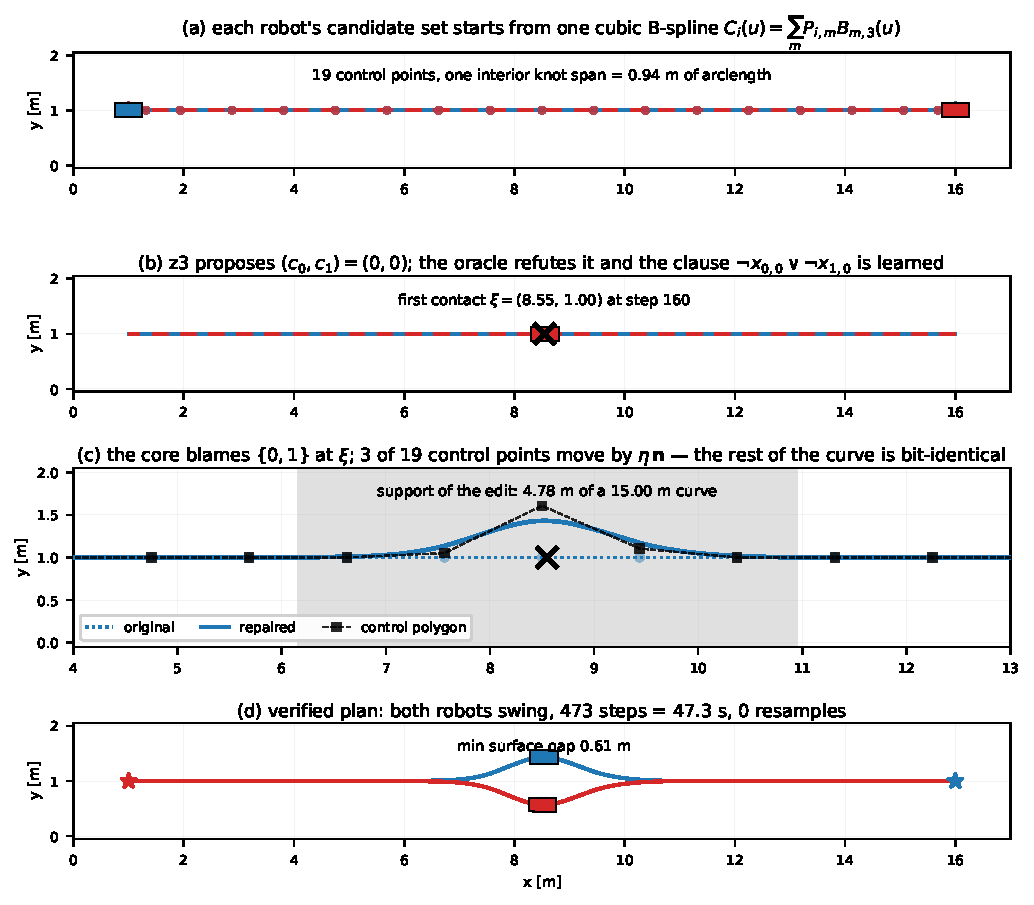
\includegraphics[width=\textwidth]{figs/worked_example.pdf}
\caption{The complete loop on the lower row of \texttt{open\_cross\_4} (the upper row is
its mirror image and is resolved identically in round 2). Robot $0$ is blue, robot $1$ red
and dashed; starts are drawn as bodies, goals as stars.
\textbf{(a)} Each robot's candidate set is seeded from one clamped cubic B-spline fitted to
a sampled guide: $19$ control points (dots) over a $23$-entry knot vector.
\textbf{(b)} z3's first model selects the fastest candidate for both robots; the oracle
refutes it at $\xi = (8.55, 1.00)$ (cross) and the clause
$\neg x_{0,0}\vee\neg x_{1,0}$ is learned. Bodies are drawn at the moment of closest
approach.
\textbf{(c)} After the unsat core blames $\{0,1\}$, the repair operator displaces the $3$
control points within $\varrho_r = 1.218$\,m of $\xi$ perpendicular to the control polygon.
The shaded band is the support of the edit: $4.78$\,m of a $15.00$\,m curve changes; the
rest is bit-identical (Prop.~\ref{prop:locality}). Vertical scale exaggerated.
\textbf{(d)} The verified plan. Both robots swing, in opposite directions, passing at
$0.61$\,m of surface clearance; $473$ steps, and the sampler was never called again.}
\label{fig:worked}
\end{figure*}

\subsection{What the example demonstrates}

\begin{itemize}
  \item \textbf{The core localises correctly.} On an instance with a known conflict
        structure, the core named exactly the pair responsible, in both rounds, without ever
        being told the rows were independent.
  \item \textbf{Repair is local and additive.} $3$ of $19$ control points moved; $68\%$ of
        the curve was untouched; every clause learned in round 1 remained valid, and in
        round 2 they alone sufficed.
  \item \textbf{Resampling was never needed.} $32$ repairs, $0$ resamples. After the initial
        guides the sampling-based planner is not consulted again --- the geometry is
        refined by proof, not by re-randomisation.
  \item \textbf{The encoding, not a heuristic, chose the asymmetry.} Robot $3$ paid nothing;
        robot $2$ paid everything. There is no priority order in the method to have produced
        that.
\end{itemize}

\section{Implementation and Parameters}

The method is implemented in Python with \texttt{scipy} for spline evaluation and z3
\cite{z3} as the solver. Table~\ref{tab:params} lists every parameter and its default.
Three of them have non-obvious roles, discussed above:
$\Delta s_{\text{ctrl}}$ is the spatial resolution of repair (Remark~\ref{rem:knots});
$\varrho_r$ sets how much of a curve one repair may rewrite; and $\lambda$ is a legal move
only because of Prop.~\ref{prop:scale}.

\begin{table}[t]
\caption{Parameters and defaults.}
\label{tab:params}
\centering
\small
\begin{tabular}{llr}
\toprule
symbol & meaning & default \\
\midrule
$\Delta s_{\text{ctrl}}$ & arclength per control point & $1.0$\,m \\
--- & curve samples per candidate & $600$ \\
$\lambda$ & slowed-variant time scale & $1.6$ \\
$w$ & en-route wait lengths & $\{30, 80\}$ steps \\
$w_{\text{long}}$ & repair wait length & $200$ steps \\
$\varrho_r/b$ & repair reach, in body units & $2.0$ \\
$N_r$ & round cap & $60$ \\
--- & bisection probes & $12$ \\
$\clr$ & required surface clearance & $0.05$\,m \\
$(k_\theta, k_v)$ & tracking gains, \eqref{eq:ff-a}--\eqref{eq:ff-al} & $(1.6, 1.2)$ \\
\bottomrule
\end{tabular}
\end{table}

\section{Limitations}
\label{sec:limits}

\paragraph*{Discrete-time collision semantics}
Stated in full in Remark~\ref{rem:gap}. This is the most important open item and it has a
known fix.

\paragraph*{Local repair cannot express a global convention}
The failure mode is instructive and we report it rather than omitting it. On a $32$-robot
instance in which every route passes through one central hub, the method does not converge:
in $1500$\,s it completes $5$ rounds, accumulates $30{,}868$ refutations, and returns core
sizes $11, 11, 7, 31$. The diagnosis is structural, not a matter of budget. A local nudge
displaces a blamed robot off a contested point and into the space another blamed robot was
simultaneously pushed towards, because each robot in the core is repaired independently. The
solution such an instance requires is a \emph{rotational convention} --- every robot going
around the hub the same way --- which is a statement about the core as a whole, not about
any robot in it. The natural next step is therefore a joint repair operator that displaces
every robot in a core to the same side of the contested point, making a roundabout emerge
from the certificate. We note that a pairwise conflict trigger structurally cannot express
this, because it never has more than two robots in scope at once; a core can.

\paragraph*{Candidate generation is heuristic}
The variant set (two speeds, two waits) and the nudge magnitudes ($\{1,2\}\times b$) are
fixed. A more principled generator would derive the displacement magnitude from the
penetration depth the oracle already computes and the wait length from the temporal overlap
at first contact, both of which are available and currently discarded.

\paragraph*{First-order and higher-dimensional models}
The realisation of Sec.~\ref{sec:realise} assumes the second-order model of
Def.~\ref{def:robot}; a first-order unicycle has no $a_{\max}$ or $\alpha_{\max}$ and needs
a different (and strictly simpler) profile stage. Extension to a second-order holonomic
model such as a planar quadrotor is direct, since flatness in the same flat outputs is
standard for that model \cite{mellinger2011}; only the flatness inverse
\eqref{eq:flatmap} changes, and the entire coordination layer is untouched.

\section{Conclusion}

We have presented a multi-robot kinodynamic planner whose coordination decisions are
triggered by proofs rather than by observed collisions. Each robot owns a growing set of
candidate motions represented as cubic B-splines, realised through the exact flatness
inverse of a second-order unicycle so that individual admissibility holds by construction;
a SAT solver selects among them under lazily learned conflict clauses; and when it proves
unsatisfiability, the unsat core names both the robots that are jointly stuck and the
workspace points at which they are stuck. B-spline local support makes acting on that
certificate a bounded, additive edit, which is what allows the learned clause database to
survive repair --- and which, on the worked instance, let one round's geometric work prove
the next round's impasse at zero cost. The clearest open problem is also the one the
certificate makes newly expressible: repairing an entire core jointly, so that a global
convention such as a roundabout can emerge from the proof rather than being hand-coded.

\section*{Reproducibility}

The worked instance of Sec.~\ref{sec:example} is \texttt{conf/env/open\_cross\_4\_unicycle2.yaml}
with \texttt{approach.method=splinecegar}; Fig.~\ref{fig:worked} and every number in
Tables~\ref{tab:result} and~\ref{tab:rounds} are produced by
\texttt{scripts/worked\_example\_fig.py} at seed $0$.

\section*{Disclosure}

Portions of the software and of this manuscript were prepared with the assistance of a
large language model. All experimental results were produced by the authors' own code and
verified by the authors; all citations were checked against their primary records before
inclusion.

\bibliographystyle{IEEEtran}
\bibliography{refs}

\end{document}
